\documentclass[11pt]{article}

% ===================== Page & Header =====================
\usepackage[a4paper, top=0.65in, bottom=0.65in, left=0.55in, right=0.55in,
            includehead]{geometry}
\usepackage{fancyhdr}
\setlength{\headheight}{15pt}
\setlength{\headsep}{20pt}
\setlength{\footskip}{14pt}
\renewcommand{\headrulewidth}{0.4pt}
\pagestyle{fancy}
\fancyhf{}
\fancyhead[L]{\normalsize FRA503 Homework 1}
\fancyhead[R]{\normalsize Chantouch, Sasish}
\fancyfoot[R]{\hspace{10pt}\thepage}

% ===================== Typography =====================
\usepackage{microtype}
\usepackage{setspace}
\usepackage{parskip}
\setlength{\parindent}{0pt}
\setlength{\parskip}{8pt}
\usepackage{setspace}
\setstretch{1.1}

% ===================== Section Styling =====================
\usepackage{titlesec}
\usepackage[table,xcdraw]{xcolor}
\definecolor{secblack}{RGB}{30,80,150}
\definecolor{secblack}{RGB}{30,30,30}
\definecolor{lightblue}{RGB}{235,242,252}
\definecolor{ruleblue}{RGB}{30,80,150}
% Named colors for TikZ figures
\definecolor{gemwhite}{RGB}{200,200,200}
\definecolor{gemred}{RGB}{210,60,60}
\definecolor{gemblue}{RGB}{60,100,200}
\definecolor{gemgreen}{RGB}{50,160,80}
\definecolor{gemblack}{RGB}{60,60,60}
\definecolor{gemgold}{RGB}{210,180,40}
\definecolor{tier3col}{RGB}{225,210,240}
\definecolor{tier2col}{RGB}{210,225,245}
\definecolor{tier1col}{RGB}{210,240,220}

\titleformat{\section}
  {\normalfont\Large\bfseries\color{secblack}}
  {\thesection}{0.6em}{}
  [\vspace{-3pt}{\color{secblue}}]
\titlespacing{\section}{0pt}{25pt}{12pt}
\titleformat{\subsection}
  {\normalfont\normalsize\bfseries\color{secblack}}
  {\thesubsection}{0.6em}{}
\titlespacing{\subsection}{0pt}{6pt}{2pt}

% ===================== Math & Science =====================
\usepackage{amsmath, amssymb}
\usepackage{cite}

% ===================== Figures & Tables =====================
\usepackage{graphicx}
\usepackage{booktabs}
\usepackage{array}
\usepackage{tabularx}
\usepackage{multirow}
\usepackage{float}
\usepackage{subcaption}
\usepackage{caption}
\captionsetup{font=small, labelfont=bf, skip=6pt}

% adjustbox: the correct tool for scaling TikZ to fit the text width
\usepackage{adjustbox}

% Float tuning — allow floats to take up to 90% of a page before
% being pushed to a dedicated float page; keep at least 10% text.
\renewcommand{\topfraction}{0.90}
\renewcommand{\bottomfraction}{0.50}
\renewcommand{\textfraction}{0.10}
\renewcommand{\floatpagefraction}{0.85}
\setcounter{topnumber}{3}
\setcounter{bottomnumber}{2}
\setcounter{totalnumber}{5}

% ===================== TikZ =====================
\usepackage{tikz}
\usetikzlibrary{shapes.geometric, arrows.meta, positioning,
                fit, backgrounds, calc, shadows.blur}

% ===================== Lists =====================
\usepackage{enumitem}
\setlist{noitemsep, topsep=2pt, partopsep=0pt}
\setlist[enumerate]{label=\arabic*.}

% ===================== Links =====================
\usepackage{hyperref}
\hypersetup{colorlinks=true, linkcolor=secblue, citecolor=secblue, urlcolor=secblue}

% ===================== Misc =====================
\usepackage{mdframed}
\newmdenv[
  backgroundcolor=lightblue,
  linecolor=secblue,
  linewidth=0.8pt,
  roundcorner=4pt,
  innerleftmargin=8pt, innerrightmargin=8pt,
  innertopmargin=5pt,  innerbottommargin=5pt,
  skipabove=4pt, skipbelow=4pt
]{infobox}

% ============================================================
\begin{document}
% ============================================================

% =================== Title Block ===================
\begin{flushleft}
  {\Large\bfseries FRA503 Deep Reinforcement Learning for Robotics}\\[10pt]
  {\large\bfseries Project Proposal: SplendorDRL with Event Based Reward Shaping and Double DQN}\\[10pt]
\end{flushleft}

\vspace{8pt}
\headrule
\vspace{10pt}

\begin{tabular}{@{}lc@{}}
\textbf{Name} & \textbf{Student ID} \\[4pt]
Chantouch Orungrote & 66340500011 \\[2pt]
Sasish Kaewsing     & 66340500076
\end{tabular}

% ============================================================
\section{Introduction}
% ============================================================

This project develops a Deep Reinforcement Learning (DRL) agent for \textit{Splendor}, a
deterministic, perfect-information, turn-based engine-building board game. Players collect
gem tokens to purchase development cards that grant permanent bonuses, with the objective
of winning the game by reaching at least 15 prestige points faster than the opponent, using the fewest turns and the fewest cards possible to break any ties. 

\section{Problem Statements}
The game presents three problems for DRL:

\begin{enumerate}
  \item \textbf{Sparse rewards} — most actions yield zero immediate prestige gain.
  \item \textbf{Delayed strategic payoff} — gem-collection and card-purchase decisions
        compound over many turns before affecting the final score.
  \item \textbf{State-dependent legal action space} — the valid action set changes every
        step based on current gem counts, visible cards, and reserved cards.
\end{enumerate}

The primary literature is \textit{Rinascimento: using event-value functions for playing
Splendor}~\cite{bravi2020}, which demonstrates that score-only evaluation is insufficient
and that event-based signals provide a richer evaluation for game-playing agents. That work
focuses on planning-based agents; this project extends the core insight into model-free DRL,
investigating whether event-based reward shaping improves a neural value learner during training.

The system supports two operational modes that share a common game environment and
real-time visualization:

\begin{center}
\renewcommand{\arraystretch}{1.25}
\begin{tabular}{>{\bfseries}p{3.2cm} p{5.0cm} p{5.2cm}}
\toprule
Mode & Description & Purpose \\
\midrule
Mode 1 — AI vs.\ AI
  & DDQN agent plays against a rule-based greedy opponent (default). The opponent
    interface is modular so future algorithms can be substituted without code changes.
  & Train and evaluate the DDQN agent under a stable, reproducible opponent. \\[4pt]
Mode 2 — AI vs.\ Human
  & A human player competes against the trained DDQN agent via a real-time graphical
    interface that highlights legal moves and renders the full game state.
  & Demonstrate learned policy quality and enable interactive inspection. \\
\bottomrule
\end{tabular}
\end{center}

\newpage

% ============================================================
\section{Objectives}
% ============================================================

\begin{itemize}
  \item Adapt an open-source \textit{Splendor} simulator into a Gym-compatible environment
        with legal action masking and a modular, swappable opponent interface.
  \item Implement a Double Deep Q-Network (DDQN) agent with experience replay, a target
        network, and masked $\varepsilon$-greedy exploration.
  \item Design an event-based reward shaping scheme with weights grounded in the primary
        literature~\cite{bravi2020} and compare it against a score-only baseline.
  \item Develop a real-time Pygame visualization supporting both AI~vs.~AI and
        AI~vs.~Human play modes, displaying all game elements necessary for full
        game understanding.
  \item Evaluate the trained agent's win rate, training stability, and sample efficiency
        against the greedy opponent under both reward conditions.
\end{itemize}

% ============================================================
\section{Scope}
% ============================================================

\begin{itemize}
    \item Standard two-player \textit{Splendor} environment
    \item Core game mechanics: gem collection, card purchase across three tiers, card reservation, noble attraction, and prestige-based victory
    \item DDQN-based learning agent with discrete action formulation and legal action masking
    \item Implementation of both operational modes
    \item Full visualization system
    \item Experimental comparison between score-only reward and event-shaped reward over random seeds
\end{itemize}
% ============================================================
\section{System Overview}
% ============================================================

The system consists of five modules. All five are active in both modes; only the Opponent
Module switches behavior between modes.

% ------------------------------------------------------------------
% Figure 1 — System Architecture
% [tp] = top of current page OR dedicated float page; never mid-text.
% adjustbox clips the TikZ to exactly \linewidth so it never overflows.
% ------------------------------------------------------------------
\begin{figure}[H]
  \centering
  \begin{adjustbox}{max width=\linewidth, center}
    \begin{tikzpicture}[
      node distance = 1.45cm and 2.2cm,
      mainbox/.style = {
        rectangle, rounded corners=5pt,
        draw=black!80, fill=lightblue,
        minimum width=3.35cm, minimum height=1.1cm,
        font=\small\bfseries, align=center, text=black,
        blur shadow={shadow blur steps=4, shadow xshift=1pt, shadow yshift=-1pt}
      },
      subbox/.style = {
        rectangle, rounded corners=5pt,
        draw=gray!55, fill=white,
        minimum width=3.2cm, minimum height=1.0cm,
        font=\small, align=center, text=black!80
      },
      arr/.style  = {-{Stealth[length=5pt,width=4pt]}, thick, color=black},
      darr/.style = {-{Stealth[length=5pt,width=4pt]}, thick, color=gray!65, dashed},
      lbl/.style  = {font=\scriptsize, text=black!75, fill=white, inner sep=1.5pt},
      note/.style = {font=\scriptsize\itshape, text=gray!80}
    ]

      % ===================== Main row =====================
      \node[mainbox] (env)   {Environment\\Module};
      \node[mainbox, right=of env] (rew)   {Reward\\Module};
      \node[mainbox, right=of rew] (agent) {DDQN Agent\\Module};

      % ===================== Lower row =====================
      \node[subbox, below=1.55cm of env]   (vis) {Visualization\\Module};
      \node[subbox, below=1.55cm of rew]   (opp) {Opponent Module\\(Greedy / Human)};
      \node[subbox, below=1.55cm of agent] (buf) {Replay\\Buffer};

      % ===================== Main training path =====================
      \draw[arr] (env.east) -- node[lbl, above] {$s_t,\ \mathrm{mask}$} (rew.west);
      \draw[arr] (rew.east) -- node[lbl, above] {$r_t$} (agent.west);

      % Action loop
      \draw[arr] (agent.north) -- ++(0,0.9) -| node[lbl, pos=0.84, above] {$a_t$} (env.north);

      % Replay buffer
      \draw[arr] (agent.south) -- node[lbl, right] {store $(s,a,r,s')$} (buf.north);
      \draw[arr] (buf.west) -- ++(-0.8,0) |- (agent.west);
      \node[lbl] at ($(buf.west)+(-0.8,0.95)$) {gradient update};

      % ===================== Interaction path =====================
      % Environment -> Visualization
      \draw[darr] (env.south) -- node[lbl, right] {game state} (vis.north);

      % Visualization -> Opponent
      \draw[darr] (vis.east) -- node[lbl, above] {human input} (opp.west);

      % Opponent -> Environment : route OUTSIDE on the far left
      \draw[darr] (opp.north) -- ++(0,0.55) -| ([xshift=-1.05cm]env.west) -- (env.west);
      \node[lbl] at ([xshift=-1.0cm,yshift=0.42cm]env.west) {opp.\ action};

      % Notes
      \node[note, right=0.22cm of buf] {training loop};
      \node[note, below=0.12cm of opp] {active in both modes};

    \end{tikzpicture}
  \end{adjustbox}
  \caption{System architecture. The main training path connects the environment,
  reward module, DDQN agent, and replay buffer. The visualization and opponent
  modules support interaction in both modes, with the opponent driven either by
  a greedy policy or by human input.}
  \label{fig:system}
\end{figure}

\subsection{State Representation}
The observation is a fixed-length normalized vector (all values in $[0,1]$) encoding the full
public game state across five groups:

\begin{center}
\renewcommand{\arraystretch}{1.15}
\begin{tabular}{lp{7.5cm}r}
\toprule
\textbf{Group} & \textbf{Content} & \textbf{Dim.} \\
\midrule
Visible cards  & 12 cards $\times$ (5 gem costs + 1 prestige + 5 bonus one-hot) & 132 \\
Noble tiles    & 3 nobles $\times$ (5 gem requirements + 1 prestige)             & 18  \\
Board supply   & 6 gem-color counts (including gold/wild)                        & 6   \\
Agent state    & 6 gem counts + 5 bonuses + $3\times11$ reserved cards + 1 prestige & 45 \\
Opponent state & 6 gem counts + 5 bonuses + 1 prestige (public info only)       & 12  \\
\midrule
\textbf{Total} & & \textbf{213} \\
\bottomrule
\end{tabular}
\end{center}

\subsection{Action Representation}
The discrete action space (size $\leq 48$) contains four action types: gem collection
($\leq 15$ legal gem combinations), card purchase (up to 15 visible or reserved cards),
card reservation (12 visible cards), and gem discard (6 colors, triggered when the 10-gem
limit is exceeded). A binary legal mask $m \in \{0,1\}^{48}$ is recomputed at every step
and applied before any $\arg\max$ selection.

\subsection{Opponent Module — Modular Design}
The Opponent Module exposes a single interface: \texttt{select\_action(obs,\,mask)}.
Any class implementing this method can be injected at environment initialization, making
the opponent fully swappable without modifying environment or training code.

\begin{itemize}
  \item \textbf{Greedy Agent (Mode~1):} selects the legal action yielding
        the highest immediate prestige; on ties, collects gems that most reduce the
        cost of the most valuable affordable card.
  \item \textbf{Human Player (Mode~2):} receives the legal mask, presents clickable
        legal options via the Visualization Module, and relays the human's selection
        back as an integer action index.
  \item \textbf{Future algorithms:} MCTS, minimax, or another DDQN can be plugged in
        by implementing \texttt{select\_action(obs,\,mask)}.
\end{itemize}

\subsection{Visualization Module}
Built with Pygame, the Visualization Module renders the complete game state in real time in
both modes. Figure~\ref{fig:vis} shows its panel layout.

% ------------------------------------------------------------------
% Figure 2 — Board-game visualization mock-up
% [p]  = dedicated float page only; keeps the large board diagram
%        entirely separate from text, eliminating any disruption.
% adjustbox scales it down to fit within the printable width.
% ------------------------------------------------------------------
\begin{figure}[H]
  \centering
  \noindent
  \begin{adjustbox}{max width=\linewidth, max height=0.88\textheight,
                    keepaspectratio, center}
    \begin{tikzpicture}[font=\scriptsize,
                        every node/.style={inner sep=1.5pt}]

      % ===================== Outer border =====================
      \draw[thick, rounded corners=6pt, color=secblue, fill=lightblue!22]
        (0,0) rectangle (15.0,6.4);

      % ===================== Panel A: Gem Supply =====================
      \draw[fill=yellow!15, rounded corners=4pt, draw=gray!50]
        (0.20,0.55) rectangle (2.35,6.15);
      \node[font=\scriptsize\bfseries, text=secblue] at (1.275,5.92) {Gem Supply};

      \foreach \y/\fc/\name in {
          5.28/gemred/Ruby,
          4.43/gemblue/Sapphire,
          3.58/gemgreen/Emerald,
          2.73/gemwhite/Diamond,
          1.88/gemblack/Onyx,
          1.03/gemgold/Gold}{
        \filldraw[\fc, draw=gray!60] (0.5,\y) circle (0.22);
        \node[anchor=west] at (0.80,\y) {\name:4};
      }

      % ===================== Panel B: Development Cards =====================
      \draw[fill=white, rounded corners=4pt, draw=gray!50]
        (2.55,0.55) rectangle (10.35,6.15);
      \node[font=\scriptsize\bfseries, text=secblue] at (6.45,5.92)
        {Development Cards --- 3 Tiers $\times$ 4 Visible};

      \foreach \row/\tierlabel/\tcolor in {
          1/{Tier 3}/tier3col,
          2/{Tier 2}/tier2col,
          3/{Tier 1}/tier1col}{
        \pgfmathsetmacro{\ybot}{5.48 - \row*1.60}
        \pgfmathsetmacro{\ytop}{\ybot+1.33}
        \node[rotate=90, font=\tiny\bfseries, text=gray]
          at (2.90,\ybot+0.665) {\tierlabel};
        \foreach \col in {1,2,3,4}{
          \pgfmathsetmacro{\xleft}{3.22 + (\col-1)*1.68}
          \pgfmathsetmacro{\xright}{\xleft+1.47}
          \draw[fill=\tcolor, rounded corners=3pt, draw=gray!60]
            (\xleft,\ybot) rectangle (\xright,\ytop);
          \node[font=\tiny] at (\xleft+0.735,\ytop-0.17) {2 pts};
          \node[font=\tiny, text=gray!80] at (\xleft+0.735,\ytop-0.43)
            {\textcolor{red!70}{\textbf{R}}2\;\textcolor{blue!60}{\textbf{S}}1};
          \node[font=\tiny, text=gray!80] at (\xleft+0.735,\ytop-0.63)
            {\textcolor{green!60!black}{\textbf{E}}0\;\textcolor{black!60}{\textbf{O}}1};
          \node[font=\tiny, fill=\tcolor!60, rounded corners=2pt]
            at (\xleft+0.735,\ybot+0.22) {Bonus: Sph.};
        }
      }

      % ===================== Right column alignment =====================
      % Noble
      \draw[fill=purple!8, rounded corners=4pt, draw=gray!50]
        (10.5,4.30) rectangle (14.8,6.15);
      \node[font=\scriptsize\bfseries, text=secblue] at (12.825,5.92) {Noble Tiles};

      \foreach \i in {0,1,2}{
        \pgfmathsetmacro{\xl}{11.12 + \i*1.18}
        \draw[fill=white, rounded corners=3pt, draw=purple!40]
          (\xl,4.58) rectangle (\xl+0.96,5.68);
        \node[font=\tiny\bfseries] at (\xl+0.48,5.48) {3 pts};
        \node[font=\tiny, text=gray] at (\xl+0.48,5.22) {R:3 E:2};
        \node[font=\tiny, text=gray] at (\xl+0.48,4.98) {S:0 D:0};
        \node[font=\tiny, text=gray] at (\xl+0.48,4.76) {O:1};
      }

      % DDQN Agent
      \draw[fill=green!10, rounded corners=4pt, draw=gray!50]
        (10.5,2.32) rectangle (14.8,4.07);
      \node[font=\scriptsize\bfseries, text=secblue] at (12.825,3.82)
        {DDQN Agent};
      \node[font=\tiny] at (12.825,3.50) {Gems: R2 S1 E0 D3 O1 G0};
      \node[font=\tiny] at (12.825,3.24) {Bonuses: R1 S0 E2 D0 O1};
      \node[font=\tiny] at (12.825,2.98) {Reserved: [Card A] [Card B] [---]};
      \node[font=\scriptsize\bfseries, text=green!60!black]
        at (12.825,2.66) {Prestige: 8 pts};

      % Opponent
      \draw[fill=orange!10, rounded corners=4pt, draw=gray!50]
        (10.5,0.55) rectangle (14.8,2.03);
      \node[font=\scriptsize\bfseries, text=secblue] at (12.825,1.78)
        {Opponent};
      \node[font=\tiny] at (12.825,1.52) {Gems: R0 S3 E1 D1 O2 G0};
      \node[font=\tiny] at (12.825,1.28) {Bonuses: R0 S2 E1 D1 O0};
      \node[font=\scriptsize\bfseries, text=orange!70!black]
        at (12.825,0.97) {Prestige: 11 pts};

      % ===================== Status Bar =====================
      \draw[fill=secblue!10, rounded corners=3pt, draw=secblue!35]
        (0.28,0.08) rectangle (14.85,0.40);
      \node[font=\tiny] at (7.56,0.24)
        {Turn 14 $\mid$ Agent's turn $\mid$
         Last action: \textit{Purchased Tier-2 Sapphire card (+2\,pts)}
         $\mid$ \textcolor{green!60!black}{\textbf{Legal moves highlighted}}};

    \end{tikzpicture}
  \end{adjustbox}
  \caption{Visualization panel layout.}
  \label{fig:vis}
\end{figure}

% ============================================================
\section{Techniques}
% ============================================================

\subsection{Double Deep Q-Network (DDQN)}
DDQN~\cite{vanhasselt2016} reduces the overestimation bias of standard DQN, which is
particularly harmful in sparse long-horizon tasks. The Bellman update target is:
\[
  y_t = r_t + \gamma\,Q\!\left(s_{t+1},\;
        \arg\max_{a'}Q_{\text{masked}}(s_{t+1},a';\theta);\;\theta^{-}\right)
\]
where $\theta$ are the online network parameters and $\theta^{-}$ are the target network
parameters, updated by a hard copy every $C=200$ steps. The network loss over a mini-batch
$\mathcal{B}$ is:
\[
  \mathcal{L}(\theta)=
  \mathbb{E}_{(s,a,r,s')\sim\mathcal{B}}\!\left[\bigl(y_t-Q(s,a;\theta)\bigr)^2\right]
\]
The online network is a three-layer MLP:
Input$(213)$\,$\to$\,FC$(256,\text{ReLU})$\,$\to$\,FC$(128,\text{ReLU})$\,$\to$\,FC$(|\mathcal{A}|)$,
optimized with Adam ($\alpha=10^{-4}$).

\subsection{Experience Replay}
A circular replay buffer of capacity $10^5$ stores transitions
$(s_t,a_t,r_t,s_{t+1},m_{t+1},\text{done}_t)$~\cite{mnih2015}. Training begins
after $B_{\min}=1{,}000$ transitions. Mini-batches of size 64 are sampled uniformly
at each gradient step to decorrelate consecutive transitions and stabilize learning.

\subsection{Legal Action Masking}
At every decision step the environment provides $m\in\{0,1\}^{|\mathcal{A}|}$.
Illegal actions are excluded from both selection and bootstrapping~\cite{Huang2022}:
\[
  Q_{\text{masked}}(s,a;\theta)=
  \begin{cases}
    Q(s,a;\theta), & m_a=1 \\
    -\infty,       & m_a=0
  \end{cases}
\]

\subsection{$\varepsilon$-Greedy Exploration with Exponential Decay}
The behavior policy selects actions with $\varepsilon$-greedy exploration over the legal
action set only, with $\varepsilon$ decaying as:
\[
  \varepsilon_k = \max\!\left(\varepsilon_{\min},\;\varepsilon_0\cdot\lambda^k\right),
  \qquad \varepsilon_0=1.0,\quad\varepsilon_{\min}=0.05,\quad\lambda=0.995
\]

\subsection{Event-Based Reward Shaping}
Motivated by Bravi and Lucas~\cite{bravi2020}, event shaping densifies the learning signal
while preserving the terminal win objective. Two reward conditions are compared:

\textbf{Score-only (baseline):}
$$r_t^{\text{score}} = \Delta P_t + \beta \cdot (\mathbf{1}[\text{win}_t] - \mathbf{1}[\text{lose}_t])$$
where $\Delta P_t$ is the prestige gained and $\beta=\pm1.0$ is the win/loss terminal bonus.

\textbf{Event-shaped:}
$$r'_t = r_t^{\text{score}} + \boldsymbol{\phi}_t^\top\mathbf{w}$$
where $\boldsymbol{\phi}_t\in\{0,1\}^5$ is the binary event vector and
$\mathbf{w}$ is the fixed weight vector in Table~\ref{tab:events}.

\begin{table}[htbp]
\centering\small
\caption{Event-shaping reward components. Weights are fixed prior to training, set
proportional to the strategic hierarchy described in~\cite{bravi2020}.}
\label{tab:events}
\renewcommand{\arraystretch}{1.12}
\begin{tabular}{clcc}
\toprule
\textbf{Event} & \textbf{Description} & \textbf{Trigger} & \textbf{Weight $w_i$}\\
\midrule
$\phi_1$ & Collect gem(s)       & Gem count increases this step         & $+0.05$ \\
$\phi_2$ & Purchase a card      & A card is acquired this step          & $+0.20$ \\
$\phi_3$ & Gain a card bonus    & Any bonus-color count increases       & $+0.10$ \\
$\phi_4$ & Attract a noble      & A noble is attracted this step        & $+0.50$ \\
$\phi_5$ & Win the game         & Agent prestige $\geq 15$ at turn end  & $+1.00$ \\
\bottomrule
\end{tabular}
\end{table}

\newpage
% ============================================================
\section{Framework}
% ============================================================

\subsection{Environment Framework}
The environment is a finite episodic Markov Decision Process
$\mathcal{M}=(\mathcal{S},\mathcal{A},P,R,\gamma)$ with $\gamma=0.99$.
An open-source \textit{Splendor} simulator is adapted to a Gym-compatible interface
exposing \texttt{reset()}, \texttt{step(action)}, mask generation, terminal detection,
and reward computation. The opponent's turn is executed inside \texttt{step()} so the
agent observes only its own decision points.

\subsection{Training Framework — Mode 1 (AI vs.\ AI)}

\begin{enumerate}
  \item Initialize environment with the Greedy Opponent; initialize replay buffer and
        DDQN networks $(\theta,\theta^{-})$ with random weights.
  \item Encode observation $s_t$ and mask $m_t$; select action $a_t$ via masked
        $\varepsilon$-greedy policy.
  \item Execute $a_t$; environment runs greedy opponent internally; return
        $(s_{t+1}, m_{t+1}, r_t, \text{done})$.
  \item Compute $r_t$ from the active reward module (score-only or event-shaped).
  \item Store transition; if $|\mathcal{B}|\geq B_{\min}$, sample mini-batch and
        update $\theta$ via Adam.
  \item Every $C=200$ steps perform a hard copy $\theta\!\to\!\theta^{-}$;
        decay $\varepsilon$ at episode end.
  \item Visualization Module renders each turn at a configurable frame delay and logs
        the last action in plain text in the status bar.
\end{enumerate}

\subsection{Deployment Framework — Mode 2 (AI vs.\ Human)}

\begin{enumerate}
  \item Load trained DDQN weights $\theta$ (frozen, $\varepsilon=0$); initialize
        environment with the Human Opponent Module.
  \item Visualization renders the full board at the start of every turn.
  \item \textit{Agent turn:} DDQN selects the greedy legal action; the visualization
        highlights the chosen card or gem combination and displays the action in
        plain text before applying it.
  \item \textit{Human turn:} legal actions are highlighted in green (cards become
        clickable; gem combinations appear as buttons); the human clicks to submit a
        move, which is passed to \texttt{step()} as an integer action index.
  \item The board re-renders after every turn; game ends when either player
        reaches 15 prestige points.
  \item End screen shows the winner, final prestige scores, and a turn-by-turn
        action history.
\end{enumerate}

\section{The Experimental Setup and Evaluation}

\begin{center}
\renewcommand{\arraystretch}{1.15}
\begin{tabular}{ccc}
\toprule
\textbf{Condition} & \textbf{Reward} & \textbf{Opponent} \\
\midrule
C0 (lower bound) & —             & Random legal agent \\
C1               & Score-only    & Greedy (fixed) \\
C2               & Event-shaped  & Greedy (fixed) \\
\bottomrule
\end{tabular}
\end{center}

\newpage

C1 and C2 are each trained for 5{,}000 episodes with 2 random seeds (4 training runs total).
All conditions are evaluated in 200 greedy-play episodes ($\varepsilon=0$) against the fixed
greedy opponent. Three metrics are reported as mean $\pm$ range across seeds:

\begin{itemize}
  \item \textbf{Win rate} vs.\ the greedy opponent — the primary performance measure.
  \item \textbf{Training reward curve} — smoothed episodic return, learning
        stability and convergence speed.
  \item \textbf{Sample efficiency} — episodes to first reach a 50\% win-rate threshold.
  \item \textbf{Visual Inspection} — human validation of agent strategy via Pygame interface in Mode 2.
\end{itemize}

% ============================================================
\section{Expected Contribution}
% ============================================================

\begin{itemize}
  \item A Gym-compatible \textit{Splendor} environment with legal action masking and a
        modular opponent interface supporting rule-based and human opponents.
  \item A masked DDQN implementation providing a reproducible baseline for
        sparse-reward board-game DRL.
  \item A real-time Pygame visualization enabling full game inspection in both
        AI~vs.~AI and AI~vs.~Human modes.
  \item An event-based reward shaping design grounded in the primary literature with
        transparent, literature-motivated fixed weights.
  \item Empirical ablation results comparing score-only and event-shaped training
        under a controlled fixed-opponent setting.
\end{itemize}

% ============================================================
\section{Faced Problems and Observations}
% ============================================================
During the initial phases of training and environment formulation, several challenges and unexpected behaviors were encountered. These highlighted the nuances of formulating a multi-player board game into a single-agent Markov Decision Process (MDP).

\subsection{MDP Formulation and Action Space Masking}
One of the primary challenges was the accurate formulation of the Splendor MDP, particularly the state-action space and rule enforcement. Splendor features a dynamic action space where the legality of actions (buying cards, taking gems) depends heavily on the current state (board tokens, player wealth, and reserves). If an agent attempts an illegal move, the environment must handle it gracefully. The initial problem was that giving a negative penalty for illegal moves caused the agent to get stuck in local optima, as it was easier to do nothing than risk a penalty. To fix this, we implemented strict \textbf{Action Masking}, which zeroes out the probability of selecting an illegal action in the DDQN's output layer before the softmax or greedy selection. 

However, this masking introduced a subtle interaction with the game's discard rule. When a player exceeds 10 tokens, they are forced to discard. The mask correctly restricts the agent to only discard actions. Yet, this created a hidden problem in the MDP's timestep logic.

\subsection{The ``Cowardice'' Strategy (Reward Discounting Exploitation)}
The most significant problem observed was a classic reinforcement learning pathology that we term the \textit{Cowardice Strategy}. In Splendor, losing to the opponent yields a terminal penalty of $-10$. Because our MDP utilizes a discount factor ($\gamma=0.99$), distant penalties are mathematically less severe than immediate ones (e.g., $-10 \times 0.99^{85} = -4.25$ is better than $-10 \times 0.99^{30} = -7.39$).

When the agent (particularly under conditions C2 and C4) realized it lacked the skill to beat the strong Greedy opponent, it sought to maximize its expected return by delaying the end of the game as much as possible. It exploited the discard masking mechanism by intentionally hoarding gems (taking 3 gems per turn) to force itself over the 10-token limit. This triggered the mandatory discard phase. Because each discard action counted as an extra RL timestep returning a $0.0$ reward, the agent effectively turned one game turn into three RL timesteps (take 3 gems, discard 2). This artificially inflated the episode lengths (jumping from a baseline of $\sim30$ steps to $\sim85$ steps) and successfully discounted the inevitable loss penalty.

% ============================================================
\section{Implementations and Fixes}
% ============================================================
To address the faced problems and enhance the experimental setup, several fixes and advanced mechanisms were implemented in the final codebase.

\subsection{Advanced Architectural Enhancements}
To prevent the agent from falling into the cowardice strategy and to boost its learning capability, we introduced advanced DQN variants:
\begin{itemize}
    \item \textbf{Dueling DQN}: Separates the estimation of state-value and action-advantage, allowing the agent to learn which states are valuable independent of the action taken. This is critical in Splendor, where the board state (e.g., available cards) dictates the game's tempo.
    \item \textbf{Prioritized Experience Replay (PER)}: Replaces uniform sampling with priority-based sampling. Transitions with high Temporal Difference (TD) error are replayed more frequently, accelerating the learning of rare but crucial events like purchasing a high-tier card or gaining a Noble.
    \item \textbf{Self-Play Curriculum}: Instead of only training against a fixed Greedy opponent, the agent periodically saves its weights to a pool and plays against past versions of itself. This curriculum learning approach prevents the agent from overfitting to a specific opponent's strategy and forces it to continuously improve.
\end{itemize}

\subsection{Reward Shaping Calibration}
To provide denser signals without encouraging pathological hoarding, multiple reward profiles were implemented and tested (C0 to C6). For instance, C4 (Card Rush) completely zeroed out the reward for taking gems to discourage hoarding, while C6 (Balanced Dense) amplified all intermediate rewards to provide a stronger gradient signal in early episodes.

% ============================================================
\section{Results and Analysis}
% ============================================================
This section analyzes the empirical results generated from the test evaluations. We examine the training dynamics, the behavioral sequences, and compare the strategic outcomes across different reward shaping conditions.

\subsection{Training Dashboard and Pathology Identification}
Figure \ref{fig:dashboard} illustrates the comprehensive training dashboard. The impact of the cowardice strategy is vividly captured in the \textit{Episode Length} and \textit{Win Rate} subplots.

\begin{figure}[htbp]
    \centering
    
\includegraphics[width=1.0\textwidth]{plots/training_dashboard.png}
    \caption{Training Dashboard summarizing the learning dynamics of all conditions. Notice the spike in episode length for C2 and C4.}
    \label{fig:dashboard}
\end{figure}

For C2 (Event-shaped) and C4 (Card Rush), the episode lengths shoot up to approximately 85 steps around episode 180,000 and 135,000, respectively. Simultaneously, their win rates plummet to $0\%$, and the smoothed return converges to exactly $-10$. This quantitatively proves the mathematical exploitation of the discount factor. The agent in these conditions has completely abandoned trying to win and is strictly optimizing for game delay.

Conversely, conditions C3 (Event-shaped + Self-play + Dueling) and C6 (Balanced Dense) successfully navigate past this local optimum. C3 achieves the highest best win rate of $64.0\%$, maintaining a low and efficient episode length ($\sim32$ steps). This demonstrates that advanced network architectures (Dueling) and curriculum learning (Self-play) are essential for overcoming the sparse and delayed nature of Splendor's terminal rewards.

\subsection{Behavioral Sequences and Transition Dynamics}
To further analyze how the agent's strategy evolved, we mapped the sequence of actions taken during evaluation games against the Greedy opponent.

\begin{figure}[htbp]
    \centering
    
\includegraphics[width=1.0\textwidth]{plots/ethogram.png}
    \caption{Action Ethogram showing the sequential behavior raster across experiments.}
    \label{fig:ethogram}
\end{figure}

The \textit{Action Ethogram} (Figure \ref{fig:ethogram}) visualizes the sequence of action categories over time. In highly performant models like C3, we observe a healthy distribution of blue/cyan elements (taking gems) interspersed with green elements (buying cards). The games end relatively quickly (indicated by the black "Game ended" regions), confirming efficient point accumulation.

\begin{figure}[htbp]
    \centering
    
\includegraphics[width=1.0\textwidth]{plots/transitions.png}
    \caption{Markov Chain diagram of action transitions.}
    \label{fig:transitions}
\end{figure}

The \textit{Action Transition Diagram} (Figure \ref{fig:transitions}) reinforces this observation. For broken models experiencing the cowardice strategy, the transitions would heavily favor self-loops or gem-taking/discarding loops, confirming the hoarding behavior. For successful models (C3, C6), the transition probabilities show a balanced, forward-moving pipeline: extracting gems leads to card purchases, which occasionally leads back to gem extraction or higher-tier purchases.

\subsection{Card Purchases and Final Performance Spread}

\begin{figure}[htbp]
    \centering
    
\includegraphics[width=0.9\textwidth]{plots/card_level_purchases.png}
    \caption{Card level purchases per game comparison between Agent and Greedy opponent.}
    \label{fig:card_levels}
\end{figure}

Figure \ref{fig:card_levels} illustrates the distribution of card levels purchased. We can observe that the baseline Greedy opponent heavily prioritizes lower-level cards (L1) to quickly build an economic engine. Agents that successfully beat the Greedy opponent (such as C3) often learn a hybrid strategy—securing enough Level 1 cards to build a foundation, but actively targeting Level 2 and Level 3 cards to secure the larger prestige points required to reach the 15-point threshold efficiently.

\subsection{Extended Analysis and Future Comparisons}
\vspace{1.5cm}
\begin{center}
    \textit{[Space reserved for the integration and comparison of the remaining diagnostic plots, including the final score distribution, sample efficiency charts, and phase flow analysis.]}
\end{center}
\vspace{3cm}

% ============================================================
\section{Conclusion}
% ============================================================

This project proposes a focused, interactive DRL study of \textit{Splendor} grounded in the
insight of Bravi and Lucas~\cite{bravi2020} that score-only signals are too sparse for
effective learning in this game. Beyond the empirical training study, the system delivers two
operational modes: Mode~1 trains and evaluates the DDQN agent against a swappable greedy
opponent, and Mode~2 allows a human player to compete against the trained agent through a
clear, complete graphical interface. This combination makes the learned policy both
quantitatively evaluable and directly demonstrable, while the modular opponent design
supports straightforward future extension to stronger algorithms.

% ============================================================
\begin{thebibliography}{9}
\bibitem{bravi2020}
I. Bravi and S. M. Lucas,
``Rinascimento: using event-value functions for playing Splendor,''
in \textit{Proc. IEEE Conf. on Games (CoG)}, 2020.

\bibitem{mnih2015}
V. Mnih \textit{et al.},
``Human-level control through deep reinforcement learning,''
\textit{Nature}, vol. 518, no. 7540, pp. 529--533, 2015.

\bibitem{vanhasselt2016}
H. van Hasselt, A. Guez, and D. Silver,
``Deep reinforcement learning with Double Q-learning,''
in \textit{Proc. AAAI Conf. on Artificial Intelligence}, 2016.

\bibitem{schaul2016}
T. Schaul, J. Quan, I. Antonoglou, and D. Silver,
``Prioritized experience replay,''
in \textit{Proc. ICLR}, 2016.

\bibitem{sutton2018}
R. S. Sutton and A. G. Barto,
\textit{Reinforcement Learning: An Introduction},
2nd ed.\ MIT Press, 2018.

\bibitem{Huang2022}
S. Huang and S. Ontañón,
\textit{A Closer Look at Invalid Action Masking in Policy Gradient Algorithms},
The International FLAIRS Conference Proceedings.vol. 35, \ 2022.
\end{thebibliography}



\end{document}
